\section{$\rho_1$ cannot be a 4-transposition}

\begin{lemma}
  \label{exclude-1}
  We now assume that $\rho_0$ and $\rho_4$ are 2-transpositions.
  If $\rho_1$ is a 4-transposition, then a generator can be written as a product of other generators, and thus the generating set does not satisfy the intersection property, and the group is not a string C-group representation.
\end{lemma}

\begin{proof}
We use Method~\ref{method}.

\paragraph{}
First we choose an involution, in this case $\rho_1$. The graph with only this involution is displayed in Figure~\ref{proof-5-1}.

\begin{figure}[H]
  \begin{center}
    \begin{tikzpicture}[scale=.8]

      \begin{scope}[every node/.style={circle,draw, transform shape}]
        \node (1)  at (0,0)  {};
        \node (2)  at (2,0)  {};
        \node (3)  at (4,0)  {};
        \node (4)  at (6,0)  {};
        \node (5)  at (8,0)  {};
        \node (6)  at (10,0) {};
        \node (7)  at (12,0) {};
        \node (8)  at (14,0) {};
        \node (9)  at (16,0) {};
        \node (10) at (18,0) {};
        \node (11) at (20,0) {};
      \end{scope}

      \begin{scope}[every node/.style={fill=white, transform shape}]

        \begin{scope}[every edge/.style={draw}]
          \path (1)  edge node {$1$} (2);
          \path (3)  edge node {$1$} (4);
          \path (5)  edge node {$1$} (6);
          \path (7)  edge node {$1$} (8);
        \end{scope}
      \end{scope}

    \end{tikzpicture}
    \caption{}
    \label{proof-5-1}
  \end{center}
\end{figure}

\paragraph{}
Now we add the 2-transposition $\rho_4$ keeping in mind that $\rho_1$ and $\rho_4$ must commute. There are only three possibilities to place the two $\rho_4$ edges by Proposition~\ref{patterns-adding}.

\paragraph{}
We now apply the second part of the Method~\ref{method}. For each of those patterns we continue with the third step. The first part deals with the first pattern, an alternating square $[\rho_1, \rho_4]$, the second part with a unique double edge $(\rho_1, \rho_4)$ and the last part with two double edges $(\rho_1, \rho_4)$.

\paragraph{}
\textbf{The alternating square}\\
The starting pattern of Method~\ref{method} is this graph:

\begin{figure}[H]
  \begin{center}
    \begin{tikzpicture}[scale=.8]

      \begin{scope}[every node/.style={circle,draw, transform shape}]
        \node (1)  at (0,2)  {};
        \node (2)  at (0,0)  {};
        \node (3)  at (2,2)  {};
        \node (4)  at (2,0)  {};
        \node (5)  at (4,0)  {};
        \node (6)  at (6,0)  {};
        \node (7)  at (8,0)  {};
        \node (8)  at (10,0)  {};
        \node (9)  at (12,0)  {};
        \node (10) at (14,0)  {};
        \node (11) at (16,0) {};
      \end{scope}

      \begin{scope}[every node/.style={fill=white, transform shape}]

        \begin{scope}[every edge/.style={draw}]
          \path (1)  edge node {$1$} (2);
          \path (3)  edge node {$1$} (4);
          \path (5)  edge node {$1$} (6);
          \path (7)  edge node {$1$} (8);
          \path (1)  edge node {$4$} (3);
          \path (2)  edge node {$4$} (4);
        \end{scope}
      \end{scope}

    \end{tikzpicture}
    \caption{}
    \label{proof-5-2}
  \end{center}
\end{figure}

\paragraph{}
Now we apply the third part of the Method and try to form a connected graph by adding some edges. First we try to extend the alternating square to a sequence. We then place the two $\rho_0$ edges. Finally we add some $\rho_2$ edge to link everything.

\paragraph{}
If $\rho_4$ forms an alternating square with $\rho_1$, it must be adjacent to another alternating square by Corollary~\ref{continue-alternating-square}. The possibilities are $[\rho_1, \rho_3]$ or $[\rho_2, \rho_4]$ by Proposition~\ref{adjacent-squares}. But the last one is impossible because $\rho_4$ is a 2-transposition by Lemma~\ref{exclude-0}. Thus we have the figure~\ref{proof-5-3}.

\begin{figure}[H]
  \begin{center}
    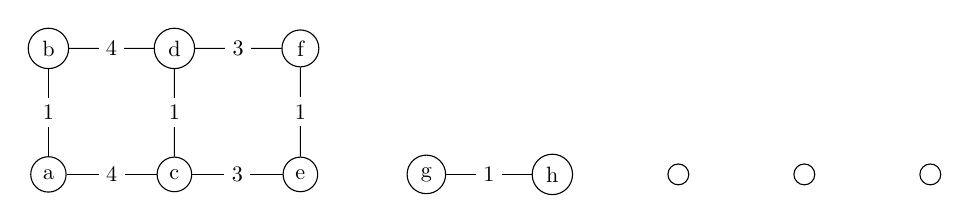
\begin{tikzpicture}[scale=.8]

      \begin{scope}[every node/.style={circle,draw, transform shape}]
        \node (1)  at (0,2)  {b};
        \node (2)  at (0,0)  {a};
        \node (3)  at (2,2)  {d};
        \node (4)  at (2,0)  {c};
        \node (5)  at (4,2)  {f};
        \node (6)  at (4,0)  {e};
        \node (7)  at (6,0)  {g};
        \node (8)  at (8,0)  {h};
        \node (9)  at (10,0) {};
        \node (10) at (12,0) {};
        \node (11) at (14,0) {};
      \end{scope}

      \begin{scope}[every node/.style={fill=white, transform shape}]

        \begin{scope}[every edge/.style={draw}]
          \path (1)  edge node {$1$} (2);
          \path (3)  edge node {$1$} (4);
          \path (5)  edge node {$1$} (6);
          \path (7)  edge node {$1$} (8);
          \path (3)  edge node {$3$} (5);
          \path (4)  edge node {$3$} (6);
          \path (1)  edge node {$4$} (3);
          \path (2)  edge node {$4$} (4);
        \end{scope}
      \end{scope}

    \end{tikzpicture}
    \caption{}
    \label{proof-5-3}
  \end{center}
\end{figure}

\paragraph{}
The sequence of squares cannot be extended to the right because two extra alternating squares are needed by Corollary~\ref{parity-sequence-squares}. If the sequence is linear, two additional $\rho_1$ edges would be used. There is only one remaining $\rho_1$ edge, therefore it is not possible to continue linearly. Also it is not possible to place the only rotation pattern found in Lemma~\ref{rotation-pattern}. The sequence cannot be extended on the right.

\paragraph{}
If the sequence is extended to the left, an alternating square $[\rho_1, \rho_3]$ is built. This uses the last $\rho_1$ edge and the last two $\rho_3$ edges. After that, only 2 $\rho_0$ edges and 2 or 4 $\rho_2$ edges remain but they cannot form a connected graph.

\paragraph{}
The sequence of alternating squares cannot be extended neither on the left nor on the right. Now we place the edges of the 2-transposition $\rho_0$.

\paragraph{}
By Lemma~\ref{adjacent-must-not-commute} $\rho_0$ and $\rho_1$ must not commute. Thus a $\rho_0$ edge must share a vertex with a $\rho_1$ edge. By Lemma~\ref{0-4-no-share}, the edges of involutions $\rho_0$ and $\rho_4$ cannot share a vertex. So the $\rho_0$ edge cannot be linked to the vertices $a, b, c$ or $d$ of Figure~\ref{proof-5-3}. Also, they cannot be adjacent to the vertices $e$ or $f$ because that would form an alternating square. But it is in contradiction with the fact that the sequence of alternating squares cannot be extended.

\paragraph{}
There are 5 acceptable vertices to place the two $\rho_0$ edges. They use 4 vertices. If one $\rho_0$ edge is connected to $g$ and the other is connected to $h$, it is impossible to make a connected graph. This component cannot be linked at all. The $g$ and $h$ vertices cannot be connected by $\rho_0$ at the same time. Hence no $\rho_1$ edge are available to connect those $\rho_0$ edge.\footnote{Clear?}

\paragraph{}
Thus either $g$ or $h$ can be used to connect a $\rho_0$ edge but not both. The case where the $\rho_0$ edge is connected to $g$ is isomorphic to the case where $\rho_0$ is connected to $h$. Thus there is only one possibility for the graph. It is displayed in Figure~\ref{proof-5-4}.

\begin{figure}[H]
  \begin{center}
    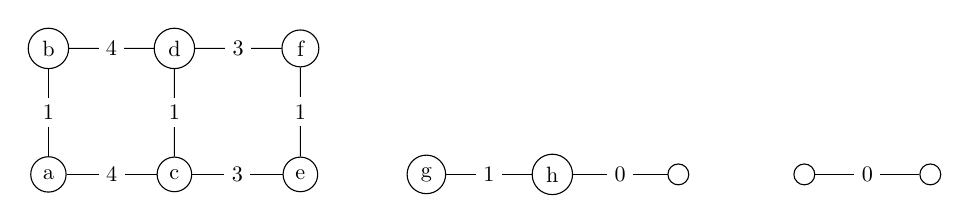
\begin{tikzpicture}[scale=.8]

      \begin{scope}[every node/.style={circle,draw, transform shape}]
        \node (1)  at (0,2)  {b};
        \node (2)  at (0,0)  {a};
        \node (3)  at (2,2)  {d};
        \node (4)  at (2,0)  {c};
        \node (5)  at (4,2)  {f};
        \node (6)  at (4,0)  {e};
        \node (7)  at (6,0)  {g};
        \node (8)  at (8,0)  {h};
        \node (9)  at (10,0) {};
        \node (10) at (12,0) {};
        \node (11) at (14,0) {};
      \end{scope}

      \begin{scope}[every node/.style={fill=white, transform shape}]

        \begin{scope}[every edge/.style={draw}]
          \path (8)  edge node {$0$} (9);
          \path (10) edge node {$0$} (11);
          \path (1)  edge node {$1$} (2);
          \path (3)  edge node {$1$} (4);
          \path (5)  edge node {$1$} (6);
          \path (7)  edge node {$1$} (8);
          \path (3)  edge node {$3$} (5);
          \path (4)  edge node {$3$} (6);
          \path (1)  edge node {$4$} (3);
          \path (2)  edge node {$4$} (4);
        \end{scope}
      \end{scope}

    \end{tikzpicture}
    \caption{}
    \label{proof-5-4}
  \end{center}
\end{figure}

\paragraph{}
We try to place the last remaining edge corresponding to $\rho_2$. By Corollary~\ref{sequence-connection}, only a single edge can be connected to the sequence of alternating squares. Moreover this edge cannot be connected to vertices $a,b,c,d$ due to Proposition~\ref{square-connection}. It must be connected to vertices $e$ or $f$ and it must be a $\rho_2$ edge by the same Lemma. But both cases are isomorphic so only one is kept.

\paragraph{}
The only available vertex to connect the other end of this $\rho_2$ edge is the point $g$.

\begin{figure}[H]
  \begin{center}
    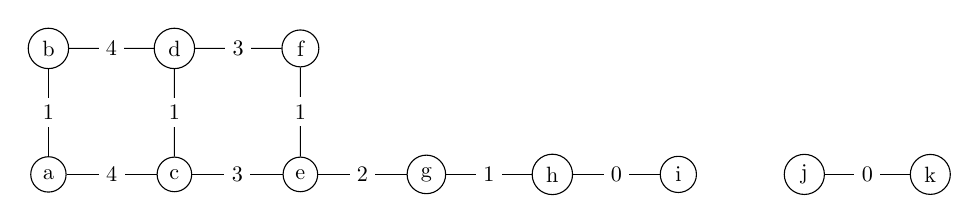
\begin{tikzpicture}[scale=.8]

      \begin{scope}[every node/.style={circle,draw, transform shape}]
        \node (1)  at (0,2)  {b};
        \node (2)  at (0,0)  {a};
        \node (3)  at (2,2)  {d};
        \node (4)  at (2,0)  {c};
        \node (5)  at (4,2)  {f};
        \node (6)  at (4,0)  {e};
        \node (7)  at (6,0)  {g};
        \node (8)  at (8,0)  {h};
        \node (9)  at (10,0)  {i};
        \node (10) at (12,0)  {j};
        \node (11) at (14,0) {k};
      \end{scope}

      \begin{scope}[every node/.style={fill=white, transform shape}]

        \begin{scope}[every edge/.style={draw}]
          \path (8)  edge node {$0$} (9);
          \path (10) edge node {$0$} (11);
          \path (1)  edge node {$1$} (2);
          \path (3)  edge node {$1$} (4);
          \path (5)  edge node {$1$} (6);
          \path (7)  edge node {$1$} (8);
          \path (6)  edge node {$2$} (7);
          \path (3)  edge node {$3$} (5);
          \path (4)  edge node {$3$} (6);
          \path (1)  edge node {$4$} (3);
          \path (2)  edge node {$4$} (4);
        \end{scope}
      \end{scope}

    \end{tikzpicture}
    \caption{}
    \label{proof-5-5}
  \end{center}
\end{figure}

\paragraph{}
All $\rho_1$ edges have been used, so they cannot be used to link the $\rho_0$ edge $(j,k)$. Therefore this edge must be part of an alternating square. This square must include the $\rho_0$ edge $(h,i)$ because it is the only other $\rho_0$ edge. The creation of the square uses two other edges of a given index. Those edge are $(h,j)$ and $(i,k)$. But the edge $(h,j)$ is adjacent to the $\rho_1$ edge $(g,h)$. Therefore, the index of the other edges of the square must be consecutive to $1$. Hence the index of the other involution of the alternating square edges must be $2$. The result can be seen in Figure~\ref{proof-5-6}.

\begin{figure}[H]
  \begin{center}
    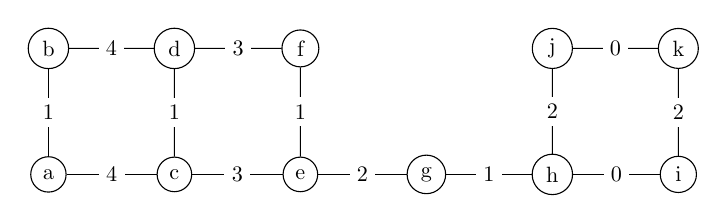
\begin{tikzpicture}[scale=.8]

      \begin{scope}[every node/.style={circle,draw, transform shape}]
        \node (1)  at (0,2)  {b};
        \node (2)  at (0,0)  {a};
        \node (3)  at (2,2)  {d};
        \node (4)  at (2,0)  {c};
        \node (5)  at (4,2)  {f};
        \node (6)  at (4,0)  {e};
        \node (7)  at (6,0)  {g};
        \node (8)  at (8,2)  {j};
        \node (9)  at (8,0)  {h};
        \node (10) at (10,2)  {k};
        \node (11) at (10,0) {i};
      \end{scope}

      \begin{scope}[every node/.style={fill=white, transform shape}]

        \begin{scope}[every edge/.style={draw}]
          \path (9)  edge node {$0$} (11);
          \path (8)  edge node {$0$} (10);
          \path (1)  edge node {$1$} (2);
          \path (3)  edge node {$1$} (4);
          \path (5)  edge node {$1$} (6);
          \path (7)  edge node {$1$} (9);
          \path (6)  edge node {$2$} (7);
          \path (8)  edge node {$2$} (9);
          \path (10) edge node {$2$} (11);
          \path (3)  edge node {$3$} (5);
          \path (4)  edge node {$3$} (6);
          \path (1)  edge node {$4$} (3);
          \path (2)  edge node {$4$} (4);
        \end{scope}
      \end{scope}

    \end{tikzpicture}
    \caption{}
    \label{proof-5-6}
  \end{center}
\end{figure}

\paragraph{}
The graph is now connected, we enter our last part of the Method: adding edges until all of them are placed.

\paragraph{}
There are only 3 $\rho_2$ edges on this graph. A last one must be added to restore parity. There are only two possible places: $(a,c)$ or $(b,d)$. That gives 2 graphs:

\begin{figure}[H]
  \begin{center}
    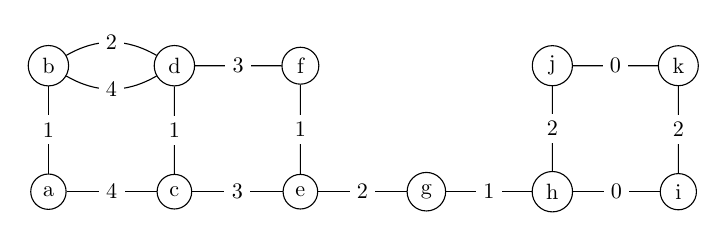
\begin{tikzpicture}[scale=.8]

      \begin{scope}[every node/.style={circle,draw, transform shape}]
        \node (1)  at (0,2)  {b};
        \node (2)  at (0,0)  {a};
        \node (3)  at (2,2)  {d};
        \node (4)  at (2,0)  {c};
        \node (5)  at (4,2)  {f};
        \node (6)  at (4,0)  {e};
        \node (7)  at (6,0)  {g};
        \node (8)  at (8,2)  {j};
        \node (9)  at (8,0)  {h};
        \node (10) at (10,2)  {k};
        \node (11) at (10,0) {i};
      \end{scope}

      \begin{scope}[every node/.style={fill=white, transform shape}]

        \begin{scope}[every edge/.style={draw}]
          \path (9)  edge node {$0$} (11);
          \path (8)  edge node {$0$} (10);
          \path (1)  edge node {$1$} (2);
          \path (3)  edge node {$1$} (4);
          \path (5)  edge node {$1$} (6);
          \path (7)  edge node {$1$} (9);
          \path (1)  edge[bend left=30] node {$2$} (3);
          \path (6)  edge node {$2$} (7);
          \path (8)  edge node {$2$} (9);
          \path (10) edge node {$2$} (11);
          \path (3)  edge node {$3$} (5);
          \path (4)  edge node {$3$} (6);
          \path (1)  edge[bend right=30] node {$4$} (3);
          \path (2)  edge node {$4$} (4);
        \end{scope}
      \end{scope}

    \end{tikzpicture}
    \caption{}
    \label{proof-5-7}
  \end{center}
\end{figure}

\begin{figure}[H]
  \begin{center}
    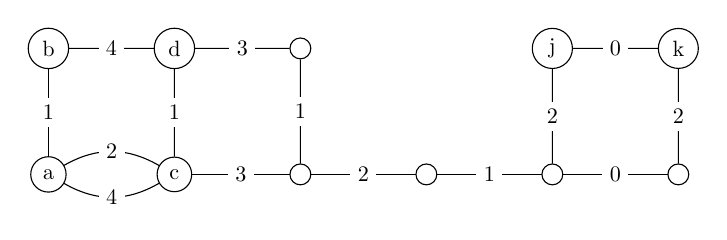
\begin{tikzpicture}[scale=.8]

      \begin{scope}[every node/.style={circle,draw, transform shape}]
        \node (1)  at (0,2)  {b};
        \node (2)  at (0,0)  {a};
        \node (3)  at (2,2)  {d};
        \node (4)  at (2,0)  {c};
        \node (5)  at (4,2)  {};
        \node (6)  at (4,0)  {};
        \node (7)  at (6,0)  {};
        \node (8)  at (8,2)  {j};
        \node (9)  at (8,0)  {};
        \node (10) at (10,2)  {k};
        \node (11) at (10,0) {};
      \end{scope}

      \begin{scope}[every node/.style={fill=white, transform shape}]

        \begin{scope}[every edge/.style={draw}]
          \path (9)  edge node {$0$} (11);
          \path (8)  edge node {$0$} (10);
          \path (1)  edge node {$1$} (2);
          \path (3)  edge node {$1$} (4);
          \path (5)  edge node {$1$} (6);
          \path (7)  edge node {$1$} (9);
          \path (2)  edge[bend left=30] node {$2$} (4);
          \path (6)  edge node {$2$} (7);
          \path (8)  edge node {$2$} (9);
          \path (10) edge node {$2$} (11);
          \path (3)  edge node {$3$} (5);
          \path (4)  edge node {$3$} (6);
          \path (1)  edge node {$4$} (3);
          \path (2)  edge[bend right=30] node {$4$} (4);
        \end{scope}
      \end{scope}

    \end{tikzpicture}
    \caption{}
    \label{proof-5-8}
  \end{center}
\end{figure}

\paragraph{}
Those graphs are valid permutation representation graphs but $\rho_3$ is a 2-transposition. To find all possibles sggis, it is needed to try to extend it to a 4-transposition. There are only two possible positions for extra $\rho_3$ edges: between $(a,b)$ and $(j,k)$. That creates two other graphs:

\begin{figure}[H]
  \begin{center}
    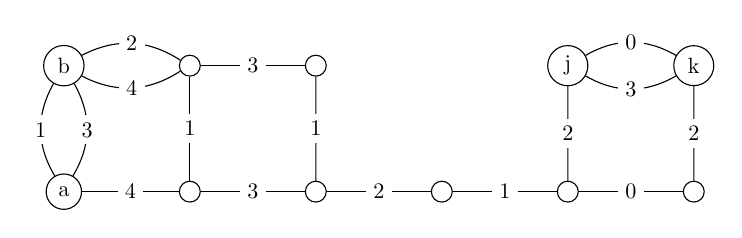
\begin{tikzpicture}[scale=.8]

      \begin{scope}[every node/.style={circle,draw, transform shape}]
        \node (1)  at (0,2)  {b};
        \node (2)  at (0,0)  {a};
        \node (3)  at (2,2)  {};
        \node (4)  at (2,0)  {};
        \node (5)  at (4,2)  {};
        \node (6)  at (4,0)  {};
        \node (7)  at (6,0)  {};
        \node (8)  at (8,2)  {j};
        \node (9)  at (8,0)  {};
        \node (10) at (10,2)  {k};
        \node (11) at (10,0) {};
      \end{scope}

      \begin{scope}[every node/.style={fill=white, transform shape}]

        \begin{scope}[every edge/.style={draw}]
          \path (9)  edge node {$0$} (11);
          \path (8)  edge[bend left=30] node {$0$} (10);
          \path (1)  edge[bend right=30] node {$1$} (2);
          \path (3)  edge node {$1$} (4);
          \path (5)  edge node {$1$} (6);
          \path (7)  edge node {$1$} (9);
          \path (1)  edge[bend left=30] node {$2$} (3);
          \path (6)  edge node {$2$} (7);
          \path (8)  edge node {$2$} (9);
          \path (10) edge node {$2$} (11);
          \path (1)  edge[bend left=30] node {$3$} (2);
          \path (3)  edge node {$3$} (5);
          \path (4)  edge node {$3$} (6);
          \path (8)  edge[bend right=30] node {$3$} (10);
          \path (1)  edge[bend right=30] node {$4$} (3);
          \path (2)  edge node {$4$} (4);
        \end{scope}
      \end{scope}

    \end{tikzpicture}
    \caption{}
    \label{proof-5-9}
  \end{center}
\end{figure}

\begin{figure}[H]
  \begin{center}
    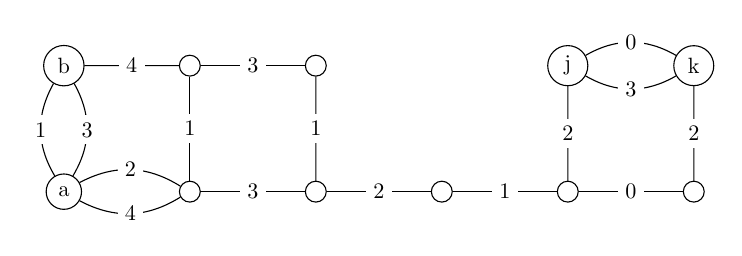
\begin{tikzpicture}[scale=.8]

      \begin{scope}[every node/.style={circle,draw, transform shape}]
        \node (1)  at (0,2)  {b};
        \node (2)  at (0,0)  {a};
        \node (3)  at (2,2)  {};
        \node (4)  at (2,0)  {};
        \node (5)  at (4,2)  {};
        \node (6)  at (4,0)  {};
        \node (7)  at (6,0)  {};
        \node (8)  at (8,2)  {j};
        \node (9)  at (8,0)  {};
        \node (10) at (10,2)  {k};
        \node (11) at (10,0) {};
      \end{scope}

      \begin{scope}[every node/.style={fill=white, transform shape}]

        \begin{scope}[every edge/.style={draw}]
          \path (9)  edge node {$0$} (11);
          \path (8)  edge[bend left=30] node {$0$} (10);
          \path (1)  edge[bend right=30] node {$1$} (2);
          \path (3)  edge node {$1$} (4);
          \path (5)  edge node {$1$} (6);
          \path (7)  edge node {$1$} (9);
          \path (2)  edge[bend left=30] node {$2$} (4);
          \path (6)  edge node {$2$} (7);
          \path (8)  edge node {$2$} (9);
          \path (10) edge node {$2$} (11);
          \path (1)  edge[bend left=30] node {$3$} (2);
          \path (3)  edge node {$3$} (5);
          \path (4)  edge node {$3$} (6);
          \path (8)  edge[bend right=30] node {$3$} (10);
          \path (1)  edge node {$4$} (3);
          \path (2)  edge[bend right=30] node {$4$} (4);
        \end{scope}
      \end{scope}

    \end{tikzpicture}
    \caption{}
    \label{proof-5-10}
  \end{center}
\end{figure}

\paragraph{}
Now we have found a set of possible permutation representation groups. But in all those four graphs, one generator can be written as a product of the other generators. To demonstrate this, we only choose some edges of the graphs.

\paragraph{}
If the $\rho_0 $ and $\rho_3$ edges are removed, all the graphs give the following one:

\begin{figure}[H]
  \begin{center}
    \begin{tikzpicture}[scale=.8]

      \begin{scope}[every node/.style={circle,draw, transform shape}]
        \node (1)  at (0,2)  {};
        \node (2)  at (0,0)  {};
        \node (3)  at (2,2)  {};
        \node (4)  at (2,0)  {};
        \node (5)  at (6,0)  {};
        \node (6)  at (4,0)  {};
        \node (7)  at (8,0)  {};
        \node (8)  at (10,0)  {};
        \node (9)  at (12,0)  {};
        \node (10) at (14,0)  {};
        \node (11) at (16,0) {};
      \end{scope}

      \begin{scope}[every node/.style={fill=white, transform shape}]

        \begin{scope}[every edge/.style={draw}]
          \path (1)  edge node {$1$} (2);
          \path (3)  edge node {$1$} (4);
          \path (5)  edge node {$1$} (6);
          \path (7)  edge node {$1$} (8);
          \path (1)  edge[bend left=30] node {$2$} (3);
          \path (5)  edge node {$2$} (7);
          \path (8)  edge node {$2$} (9);
          \path (10) edge node {$2$} (11);
          \path (1)  edge[bend right=30] node {$4$} (3);
          \path (2)  edge node {$4$} (4);
        \end{scope}
      \end{scope}

    \end{tikzpicture}
    \caption{}
    \label{proof-5-11}
  \end{center}
\end{figure}

\paragraph{}
But it can be easily seen that $\rho_4 = (\rho_1 \rho_2)^{10}$. Thus none of those four sggis are string C-group representations by Property~\ref{generators-not-free}. Thus they cannot be an automorphism group of a polytope.

\paragraph{}
\textbf{One double edge}\\
The second possibility is to have a double edge $(\rho_1, \rho_4)$. The double edge alone is too small to be used as a starting pattern for the Method~\ref{method}. By Lemma~\ref{continue-double-edge}, this double edge must be adjacent to some alternating square. The pattern that we choose includes this alternating square. By Proposition~\ref{adjacent-squares}, there are two possibilities for the alternating square: $[\rho_1, \rho_3]$ or $[\rho_2, \rho_4]$. Therefore we have 2 starting patterns.

\paragraph{}
\textit{Alternating square $[\rho_1, \rho_3]$}

\begin{figure}[H]
  \begin{center}
    \begin{tikzpicture}[scale=.8]

      \begin{scope}[every node/.style={circle,draw, transform shape}]
        \node (1)  at (0,2)  {};
        \node (2)  at (0,0)  {};
        \node (3)  at (2,2)  {};
        \node (4)  at (2,0)  {};
        \node (5)  at (4,0)  {};
        \node (6)  at (6,0)  {};
        \node (7)  at (8,0)  {};
        \node (8)  at (10,0)  {};
        \node (9)  at (12,0)  {};
        \node (10) at (14,0)  {};
        \node (11) at (16,0) {};
      \end{scope}

      \begin{scope}[every node/.style={fill=white, transform shape}]

        \begin{scope}[every edge/.style={draw}]
          \path (1)  edge[bend right=30] node {$1$} (2);
          \path (3)  edge node {$1$} (4);
          \path (5)  edge node {$1$} (6);
          \path (7)  edge node {$1$} (8);
          \path (1)  edge node {$3$} (3);
          \path (2)  edge node {$3$} (4);
          \path (1)  edge[bend left=30] node {$4$} (2);
        \end{scope}
      \end{scope}

    \end{tikzpicture}
    \caption{}
    \label{proof-5-12}
  \end{center}
\end{figure}

\paragraph{}
By lemma~\ref{adjacent-must-not-commute}, $\rho_0$ and $\rho_1$ must not commute. A $\rho_0$ edge must thus be connected to at least one $\rho_1$ edge. So at least one $\rho_1$ edge must not be part of an alternating square if there are no $\rho_0$ edges in this square.

\paragraph{}
The alternating square cannot be extended to a sequence on the right because this needs two alternating squares by Proposition~\ref{parity-sequence-squares}.  If the index of the vertical edges is not changed, adding two squares would require all of the $\rho_1$ edges. None of the horizontal edges of the squares can be an edge of $\rho_0$. Thus, the square cannot be extended to the right by the previous statement.

\paragraph{}
The values of the vertical edges must therefore be changed. There is a single pattern for a linear change of the vertical index. It has been seen in Lemma~\ref{linear-pattern}. But it cannot be applied in this case because it requires a third $\rho_4$ edge. Thus the alternating squares cannot be extended to a sequence on the right.

\paragraph{}
If an alternating square is attached on the left, it must be $[\rho_2, \rho_4]$ by Propositions~\ref{continue-double-edge} and~\ref{continue-alternating-square}.

\begin{figure}[H]
  \begin{center}
    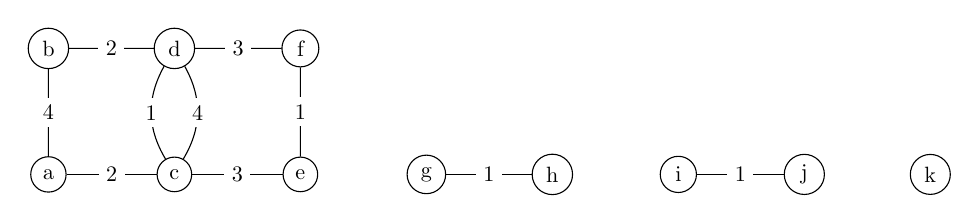
\begin{tikzpicture}[scale=.8]

      \begin{scope}[every node/.style={circle,draw, transform shape}]
        \node (1)  at (0,2)  {d};
        \node (2)  at (0,0)  {c};
        \node (3)  at (2,2)  {f};
        \node (4)  at (2,0)  {e};
        \node (5)  at (4,0)  {g};
        \node (6)  at (6,0)  {h};
        \node (7)  at (8,0)  {i};
        \node (8)  at (10,0)  {j};
        \node (9)  at (-2,2)  {b};
        \node (10) at (-2,0)  {a};
        \node (11) at (12,0) {k};
      \end{scope}

      \begin{scope}[every node/.style={fill=white, transform shape}]

        \begin{scope}[every edge/.style={draw}]
          \path (1)  edge[bend right=30] node {$1$} (2);
          \path (3)  edge node {$1$} (4);
          \path (5)  edge node {$1$} (6);
          \path (7)  edge node {$1$} (8);
          \path (1)  edge node {$2$} (9);
          \path (2)  edge node {$2$} (10);
          \path (1)  edge node {$3$} (3);
          \path (2)  edge node {$3$} (4);
          \path (1)  edge[bend left=30] node {$4$} (2);
          \path (9)  edge node {$4$} (10);
        \end{scope}
      \end{scope}

    \end{tikzpicture}
    \caption{}
    \label{proof-5-13}
  \end{center}
\end{figure}

\paragraph{}
The two $\rho_0$ edges cannot be connected to any vertex $a, b, c, d, e, f$ of the left component by Proposition~\ref{square-connection}. The point $k$ cannot be connected by two $\rho_0$ edges thus there is a single possibility to place $\rho_0$ edges up to isomorphism: link $(h, i)$ and $(j, k)$.


\begin{figure}[H]
  \begin{center}
    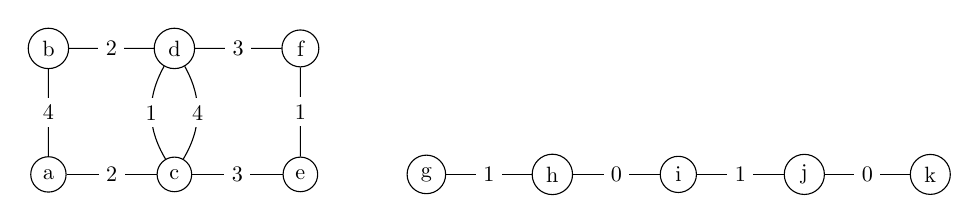
\begin{tikzpicture}[scale=.8]

      \begin{scope}[every node/.style={circle,draw, transform shape}]
        \node (1)  at (0,2)  {d};
        \node (2)  at (0,0)  {c};
        \node (3)  at (2,2)  {f};
        \node (4)  at (2,0)  {e};
        \node (5)  at (4,0)  {g};
        \node (6)  at (6,0)  {h};
        \node (7)  at (8,0)  {i};
        \node (8)  at (10,0)  {j};
        \node (9)  at (-2,2)  {b};
        \node (10) at (-2,0)  {a};
        \node (11) at (12,0) {k};
      \end{scope}

      \begin{scope}[every node/.style={fill=white, transform shape}]

        \begin{scope}[every edge/.style={draw}]
          \path (6)  edge node {$0$} (7);
          \path (8)  edge node {$0$} (11);
          \path (1)  edge[bend right=30] node {$1$} (2);
          \path (3)  edge node {$1$} (4);
          \path (5)  edge node {$1$} (6);
          \path (7)  edge node {$1$} (8);
          \path (1)  edge node {$2$} (9);
          \path (2)  edge node {$2$} (10);
          \path (1)  edge node {$3$} (3);
          \path (2)  edge node {$3$} (4);
          \path (1)  edge[bend left=30] node {$4$} (2);
          \path (9)  edge node {$4$} (10);
        \end{scope}
      \end{scope}

    \end{tikzpicture}
    \caption{}
  \end{center}
\end{figure}

\paragraph{}
By Proposition~\ref{chain-consecutive}, the component $\{g,h,i,j,k\}$ can only be connected by a $\rho_2$ edge on the vertex $g$ as all $\rho_0$ have been used. Nothing can be connected to the vertex $k$ because a $\rho_1$ edge is needed but none are available. On the other component a $\rho_2$ edge can only be attached to $e$ or $f$ by Property~\ref{fixed-only-1}.

\begin{figure}[H]
  \begin{center}
    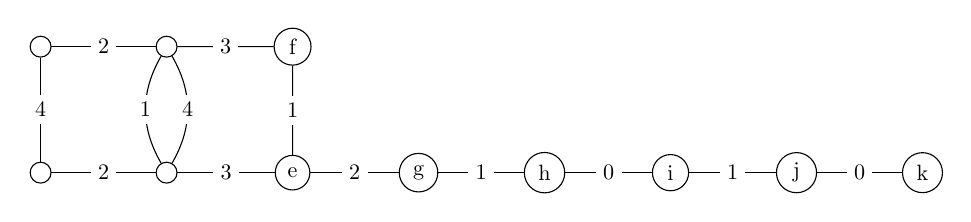
\begin{tikzpicture}[scale=.8]

      \begin{scope}[every node/.style={circle,draw, transform shape}]
        \node (1)  at (0,2)  {};
        \node (2)  at (0,0)  {};
        \node (3)  at (2,2)  {f};
        \node (4)  at (2,0)  {e};
        \node (5)  at (4,0)  {g};
        \node (6)  at (6,0)  {h};
        \node (7)  at (8,0)  {i};
        \node (8)  at (10,0)  {j};
        \node (9)  at (-2,2)  {};
        \node (10) at (-2,0)  {};
        \node (11) at (12,0) {k};
      \end{scope}

      \begin{scope}[every node/.style={fill=white, transform shape}]

        \begin{scope}[every edge/.style={draw}]
          \path (8)  edge node {$0$} (11);
          \path (6)  edge node {$0$} (7);
          \path (1)  edge[bend right=30] node {$1$} (2);
          \path (3)  edge node {$1$} (4);
          \path (5)  edge node {$1$} (6);
          \path (7)  edge node {$1$} (8);
          \path (1)  edge node {$2$} (9);
          \path (2)  edge node {$2$} (10);
          \path (4)  edge node {$2$} (5);
          \path (1)  edge node {$3$} (3);
          \path (2)  edge node {$3$} (4);
          \path (1)  edge[bend left=30] node {$4$} (2);
          \path (9)  edge node {$4$} (10);
        \end{scope}
      \end{scope}

    \end{tikzpicture}
    \caption{}
  \end{center}
\end{figure}

\paragraph{}
The graph is now connected. We begin the last part of the method~\ref{method}: place all remaining edges to satisfy parity. Thus at least one $\rho_2$ edge must still be placed. The only available vertices are $f,h,i,j$ and $k$. But $f$ cannot be connected to any other point by a $\rho_0$ edge because it must form an alternating square but that would not satisfy Proposition~\ref{adjacent-squares}. Thus an edge $(h,i)$ or an edge $(j,k)$ must be built. That gives us two cases.

\begin{figure}[H]
  \begin{center}
    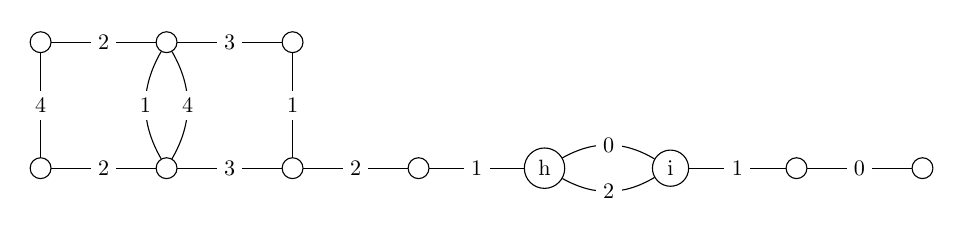
\begin{tikzpicture}[scale=.8]

      \begin{scope}[every node/.style={circle,draw, transform shape}]
        \node (1)  at (0,2)  {};
        \node (2)  at (0,0)  {};
        \node (3)  at (2,2)  {};
        \node (4)  at (2,0)  {};
        \node (5)  at (4,0)  {};
        \node (6)  at (6,0)  {h};
        \node (7)  at (8,0)  {i};
        \node (8)  at (10,0)  {};
        \node (9)  at (-2,2)  {};
        \node (10) at (-2,0)  {};
        \node (11) at (12,0) {};
      \end{scope}

      \begin{scope}[every node/.style={fill=white, transform shape}]

        \begin{scope}[every edge/.style={draw}]
          \path (6)  edge[bend left=30] node {$0$} (7);
          \path (8)  edge node {$0$} (11);
          \path (1)  edge[bend right=30] node {$1$} (2);
          \path (3)  edge node {$1$} (4);
          \path (5)  edge node {$1$} (6);
          \path (7)  edge node {$1$} (8);
          \path (1)  edge node {$2$} (9);
          \path (2)  edge node {$2$} (10);
          \path (4)  edge node {$2$} (5);
          \path (6)  edge[bend right=30] node {$2$} (7);
          \path (1)  edge node {$3$} (3);
          \path (2)  edge node {$3$} (4);
          \path (1)  edge[bend left=30] node {$4$} (2);
          \path (9)  edge node {$4$} (10);
        \end{scope}
      \end{scope}

    \end{tikzpicture}
    \caption{}
  \end{center}
\end{figure}

\begin{figure}[H]
  \begin{center}
    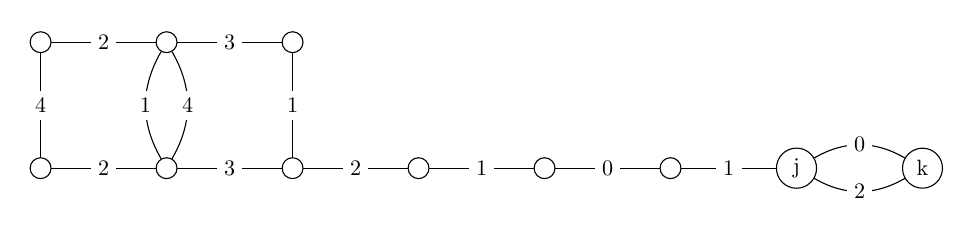
\begin{tikzpicture}[scale=.8]

      \begin{scope}[every node/.style={circle,draw, transform shape}]
        \node (1)  at (0,2)  {};
        \node (2)  at (0,0)  {};
        \node (3)  at (2,2)  {};
        \node (4)  at (2,0)  {};
        \node (5)  at (4,0)  {};
        \node (6)  at (6,0)  {};
        \node (7)  at (8,0)  {};
        \node (8)  at (10,0)  {j};
        \node (9)  at (-2,2)  {};
        \node (10) at (-2,0)  {};
        \node (11) at (12,0) {k};
      \end{scope}

      \begin{scope}[every node/.style={fill=white, transform shape}]

        \begin{scope}[every edge/.style={draw}]
          \path (6)  edge node {$0$} (7);
          \path (8)  edge[bend left=30] node {$0$} (11);
          \path (1)  edge[bend right=30] node {$1$} (2);
          \path (3)  edge node {$1$} (4);
          \path (5)  edge node {$1$} (6);
          \path (7)  edge node {$1$} (8);
          \path (1)  edge node {$2$} (9);
          \path (2)  edge node {$2$} (10);
          \path (4)  edge node {$2$} (5);
          \path (8)  edge[bend right=30] node {$2$} (11);
          \path (1)  edge node {$3$} (3);
          \path (2)  edge node {$3$} (4);
          \path (1)  edge[bend left=30] node {$4$} (2);
          \path (9)  edge node {$4$} (10);
        \end{scope}
      \end{scope}

    \end{tikzpicture}
    \caption{}
  \end{center}
\end{figure}

\paragraph{}
Now we want to prove that one generator can be written as a product of the other. The strategy used is different because there is no obvious solution. We remove one involution and then prove that the generated group is still $A_{11}$. But the removed generator is in $A_{11}$ thus it must be written as a product of other generators.

\paragraph{}
To achieve this goal, we use the classification of primitive groups. Those groups are well-known and have been classified in~\cite{buekenhout1996list} for groups of degree smaller than 50. We first prove that the group is 2-transitive with Proposition~\ref{practical-transitivity}. We then use Property~\ref{2-transitive-primitive} to prove that they are primitive.

\paragraph{}
We must have some hints about the order of the group in order to eliminate possible groups from the classification~\cite{buekenhout1996list}. To do this, we use Property~\ref{magic-formula} to know that the order of the group must be a multiple of the order of each of its subgroups.

\paragraph{}
In the first graph we remove the $\rho_4$ edges. The graph becomes the following.

\begin{figure}[H]
  \begin{center}
    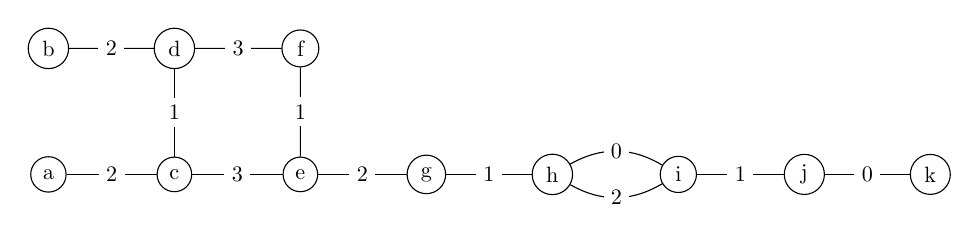
\begin{tikzpicture}[scale=.8]

      \begin{scope}[every node/.style={circle,draw, transform shape}]
        \node (1)  at (0,2)  {d};
        \node (2)  at (0,0)  {c};
        \node (3)  at (2,2)  {f};
        \node (4)  at (2,0)  {e};
        \node (5)  at (4,0)  {g};
        \node (6)  at (6,0)  {h};
        \node (7)  at (8,0)  {i};
        \node (8)  at (10,0)  {j};
        \node (9)  at (-2,2)  {b};
        \node (10) at (-2,0)  {a};
        \node (11) at (12,0) {k};
      \end{scope}

      \begin{scope}[every node/.style={fill=white, transform shape}]

        \begin{scope}[every edge/.style={draw}]
          \path (6)  edge[bend left=30] node {$0$} (7);
          \path (8)  edge node {$0$} (11);
          \path (1)  edge node {$1$} (2);
          \path (3)  edge node {$1$} (4);
          \path (5)  edge node {$1$} (6);
          \path (7)  edge node {$1$} (8);
          \path (1)  edge node {$2$} (9);
          \path (2)  edge node {$2$} (10);
          \path (4)  edge node {$2$} (5);
          \path (6)  edge[bend right=30] node {$2$} (7);
          \path (1)  edge node {$3$} (3);
          \path (2)  edge node {$3$} (4);
        \end{scope}
      \end{scope}

    \end{tikzpicture}
    \caption{}
  \end{center}
\end{figure}

\paragraph{}
The graph is connected, thus the group is transitive on 11 points. Moreover, this group is 2-transitive. To prove this we use the Proposition~\ref{practical-transitivity}: we fix the point $k$ and try to keep $k$ fixed while finding permutation between $j$ and all non-fixed point. But this is trivial because the point $k$ does not move if no $\rho_0$ edges are placed. But all the other points are in the same orbit of $\Gamma_{\rho_1, \rho_2, \rho_3}$ and thus $j$ can be permuted with any non-fixed point without using a $\rho_0$ edge.

\paragraph{}
The group is 2-transitive thus primitive. Its order is a multiple of $11 \times 10 = 110$. The subgroup $\Gamma_{\rho_2, \rho_3}$ is $D_{24}$. Thus the order of the group must be a multiple of 1320. There are 3 possibilities in~\cite{buekenhout1996list}: $M_{11}$, $A_{11}$ and $S_{11}$. $M_{11}$ is not possible because $D_{24}$ is not a subgroup of $M_{11}$, see for instance~\cite{connor2013atlas}. All involutions are even and $S_{11}$ contains odd involutions. Therefore the group must be $A_{11}$.

\paragraph{}
$\rho_4 \in A_{11}$, thus $\rho_4$ can be written as a product of other generators. Thus the set of generators is not free and cannot be a string C-group representation of $A_{11}$.\footnote{One case missing}

\paragraph{}
\textit{Alternating square $[\rho_2,\rho_4]$}

\begin{figure}[H]
  \begin{center}
    \begin{tikzpicture}[scale=.8]

      \begin{scope}[every node/.style={circle,draw, transform shape}]
        \node (1)  at (0,2)  {};
        \node (2)  at (0,0)  {};
        \node (3)  at (2,2)  {};
        \node (4)  at (2,0)  {};
        \node (5)  at (6,0)  {};
        \node (6)  at (4,0)  {};
        \node (7)  at (10,0)  {};
        \node (8)  at (8,0)  {};
        \node (9)  at (12,0)  {};
        \node (10) at (14,0)  {};
        \node (11) at (16,0) {};
      \end{scope}

      \begin{scope}[every node/.style={fill=white, transform shape}]

        \begin{scope}[every edge/.style={draw}]
          \path (1)  edge[bend right=30] node {$1$} (2);
          \path (5)  edge node {$1$} (6);
          \path (7)  edge node {$1$} (8);
          \path (9)  edge node {$1$} (10);
          \path (1)  edge node {$2$} (3);
          \path (2)  edge node {$2$} (4);
          \path (1)  edge[bend left=30] node {$4$} (2);
          \path (3)  edge node {$4$} (4);
        \end{scope}
      \end{scope}

    \end{tikzpicture}
    \caption{}
  \end{center}
\end{figure}

\paragraph{}
As usual we try to place another square next to the first one to build a sequence of alternating squares. If the new square is placed on the right, there are two possibilities i.e. change the indices of vertical edges or not. But they cannot be changed because, by Proposition~\ref{linear-pattern}, a $\rho_1$ edge is needed but all of its edges have already been placed. If the index is not changed a third $\rho_4$ edge is needed but that it impossible because $\rho_4$ is a 2-transposition. Thus no sequence can be built on the right.

\paragraph{}
A sequence of alternating squares can however be built on the left. The alternating square must be extended in a sequence to the left by a $[\rho_1, \rho_3]$ square but this case has already been seen in Figure~\ref{proof-5-13}.

\paragraph{}
The only remaining possibility is to link the square to the rest of the graph with a single edge. A $\rho_3$ edge must be used by Lemma~\ref{square-connection}. This edge cannot be adjacent to a $\rho_1$ edge otherwise an alternating square must be built. This new square forms a sequence with the square $[\rho_2, \rho_4]$ and we proved that this square cannot be extended. Thus the $\rho_3$ edge must be connected to the fixed point.

\begin{figure}[H]
  \begin{center}
    \begin{tikzpicture}[scale=.8]

      \begin{scope}[every node/.style={circle,draw, transform shape}]
        \node (1)  at (0,2)  {b};
        \node (2)  at (0,0)  {a};
        \node (3)  at (2,2)  {d};
        \node (4)  at (2,0)  {c};
        \node (5)  at (8,0)  {};
        \node (6)  at (6,0)  {};
        \node (7)  at (12,0)  {};
        \node (8)  at (10,0)  {};
        \node (9)  at (14,0)  {};
        \node (10) at (16,0)  {};
        \node (11) at (4,0) {e};
      \end{scope}

      \begin{scope}[every node/.style={fill=white, transform shape}]

        \begin{scope}[every edge/.style={draw}]
          \path (1)  edge[bend right=30] node {$1$} (2);
          \path (5)  edge node {$1$} (6);
          \path (7)  edge node {$1$} (8);
          \path (9)  edge node {$1$} (10);
          \path (1)  edge node {$2$} (3);
          \path (2)  edge node {$2$} (4);
          \path (4)  edge node {$3$} (11);
          \path (1)  edge[bend left=30] node {$4$} (2);
          \path (3)  edge node {$4$} (4);
        \end{scope}
      \end{scope}

    \end{tikzpicture}
    \caption{}
  \end{center}
\end{figure}

\paragraph{}
Two $\rho_0$ edges must still be placed and they must not commute with $\rho_1$. Thus at least one edge must be adjacent to a $\rho_1$ edge. However the other end of the edge cannot be connected to either $a,b,c,d$ or $e$ by Proposition~\ref{square-connection} or by Proposition~\ref{chain-consecutive}. This $\rho_1$ edge must thus be adjacent to two $\rho_0$ edges. Moreover the other $\rho_0$ edge must also link the two other $\rho_1$ edges.

\begin{figure}[H]
  \begin{center}
    \begin{tikzpicture}[scale=.8]

      \begin{scope}[every node/.style={circle,draw, transform shape}]
        \node (1)  at (0,2)  {};
        \node (2)  at (0,0)  {};
        \node (3)  at (2,2)  {};
        \node (4)  at (2,0)  {};
        \node (5)  at (8,0)  {};
        \node (6)  at (6,0)  {};
        \node (7)  at (12,0)  {};
        \node (8)  at (10,0)  {};
        \node (9)  at (14,0)  {};
        \node (10) at (16,0)  {};
        \node (11) at (4,0) {};
      \end{scope}

      \begin{scope}[every node/.style={fill=white, transform shape}]

        \begin{scope}[every edge/.style={draw}]
          \path (5)  edge node {$0$} (8);
          \path (7)  edge node {$0$} (9);
          \path (1)  edge[bend right=30] node {$1$} (2);
          \path (5)  edge node {$1$} (6);
          \path (7)  edge node {$1$} (8);
          \path (9)  edge node {$1$} (10);
          \path (1)  edge node {$2$} (3);
          \path (2)  edge node {$2$} (4);
          \path (4)  edge node {$3$} (11);
          \path (1)  edge[bend left=30] node {$4$} (2);
          \path (3)  edge node {$4$} (4);
        \end{scope}
      \end{scope}

    \end{tikzpicture}
    \caption{}
  \end{center}
\end{figure}

\paragraph{}
By Proposition~\ref{chain-consecutive} and since all $\rho_4$ edges have been used and since no $\rho_2$ can be connected to the alternating square, a $\rho_2$ edge must be used to connect the two components together.

\begin{figure}[H]
  \begin{center}
    \begin{tikzpicture}[scale=.8]

      \begin{scope}[every node/.style={circle,draw, transform shape}]
        \node (1)  at (0,2)  {b};
        \node (2)  at (0,0)  {a};
        \node (3)  at (2,2)  {};
        \node (4)  at (2,0)  {};
        \node (5)  at (8,0)  {g};
        \node (6)  at (6,0)  {};
        \node (7)  at (12,0)  {i};
        \node (8)  at (10,0)  {h};
        \node (9)  at (14,0)  {j};
        \node (10) at (16,0)  {};
        \node (11) at (4,0) {};
      \end{scope}

      \begin{scope}[every node/.style={fill=white, transform shape}]

        \begin{scope}[every edge/.style={draw}]
          \path (5)  edge node {$0$} (8);
          \path (7)  edge node {$0$} (9);
          \path (1)  edge[bend right=30] node {$1$} (2);
          \path (5)  edge node {$1$} (6);
          \path (7)  edge node {$1$} (8);
          \path (9)  edge node {$1$} (10);
          \path (1)  edge node {$2$} (3);
          \path (2)  edge node {$2$} (4);
          \path (11)  edge node {$2$} (6);
          \path (4)  edge node {$3$} (11);
          \path (1)  edge[bend left=30] node {$4$} (2);
          \path (3)  edge node {$4$} (4);
        \end{scope}
      \end{scope}

    \end{tikzpicture}
    \caption{}
  \end{center}
\end{figure}

\paragraph{}
The $\rho_3$ involution is currently odd. An extra $\rho_3$ edge must be placed. The only possibility is $(a,b)$. The missing $\rho_2$ edge must then be placed such that a $\rho_0$ edge is doubled i.e $(g,h)$ or $(i,j)$. That gives us are two graphs displayed in figure~\ref{proof-5-23} and~\ref{proof-5-24}.


\begin{figure}[H]
  \begin{center}
    \begin{tikzpicture}[scale=.8]

      \begin{scope}[every node/.style={circle,draw, transform shape}]
        \node (1)  at (0,2)  {b};
        \node (2)  at (0,0)  {a};
        \node (3)  at (2,2)  {};
        \node (4)  at (2,0)  {};
        \node (5)  at (8,0)  {};
        \node (6)  at (6,0)  {};
        \node (7)  at (12,0)  {};
        \node (8)  at (10,0)  {};
        \node (9)  at (14,0)  {};
        \node (10) at (16,0)  {};
        \node (11) at (4,0) {};
      \end{scope}

      \begin{scope}[every node/.style={fill=white, transform shape}]

        \begin{scope}[every edge/.style={draw}]
          \path (5)  edge[bend left=30] node {$0$} (8);
          \path (7)  edge node {$0$} (9);
          \path (1)  edge[bend right=40] node {$1$} (2);
          \path (5)  edge node {$1$} (6);
          \path (7)  edge node {$1$} (8);
          \path (9)  edge node {$1$} (10);
          \path (1)  edge node {$2$} (3);
          \path (2)  edge node {$2$} (4);
          \path (5)  edge[bend right=30] node {$2$} (8);
          \path (11) edge node {$2$} (6);
          \path (1)  edge node {$3$} (2);
          \path (4)  edge node {$3$} (11);
          \path (1)  edge[bend left=40] node {$4$} (2);
          \path (3)  edge node {$4$} (4);
        \end{scope}
      \end{scope}

    \end{tikzpicture}
    \caption{}
    \label{proof-5-23}
  \end{center}
\end{figure}

\begin{figure}[H]
  \begin{center}
    \begin{tikzpicture}[scale=.8]

      \begin{scope}[every node/.style={circle,draw, transform shape}]
        \node (1)  at (0,2)  {};
        \node (2)  at (0,0)  {};
        \node (3)  at (2,2)  {};
        \node (4)  at (2,0)  {};
        \node (5)  at (8,0)  {};
        \node (6)  at (6,0)  {};
        \node (7)  at (12,0)  {};
        \node (8)  at (10,0)  {};
        \node (9)  at (14,0)  {};
        \node (10) at (16,0)  {};
        \node (11) at (4,0) {};
      \end{scope}

      \begin{scope}[every node/.style={fill=white, transform shape}]

        \begin{scope}[every edge/.style={draw}]
          \path (5)  edge node {$0$} (8);
          \path (7)  edge[bend left=30] node {$0$} (9);
          \path (1)  edge[bend right=40] node {$1$} (2);
          \path (5)  edge node {$1$} (6);
          \path (7)  edge node {$1$} (8);
          \path (9)  edge node {$1$} (10);
          \path (1)  edge node {$2$} (3);
          \path (2)  edge node {$2$} (4);
          \path (7)  edge[bend right=30] node {$2$} (9);
          \path (11) edge node {$2$} (6);
          \path (1)  edge node {$3$} (2);
          \path (4)  edge node {$3$} (11);
          \path (1)  edge[bend left=40] node {$4$} (2);
          \path (3)  edge node {$4$} (4);
        \end{scope}
      \end{scope}

    \end{tikzpicture}
    \caption{}
    \label{proof-5-24}
  \end{center}
\end{figure}

\paragraph{}
There are no possibility to convert $\rho_3$ to a 4-transposition in this case.

\paragraph{}
If the $\rho_0$ and $\rho_3$ edges are removed, we get back the graph displayed in Figure~\ref{proof-5-11}. Thus the same conclusion applies and none of the sggis of Figures~\ref{proof-5-23} and~\ref{proof-5-24} are string C-groups representations of $A_{11}$.

\paragraph{}
\textbf{Two double edges}\\
The double edges must be contained into alternating squares by Lemma~\ref{continue-double-edge}. There are two possibilities depending if the two double edges are in the same alternating square or not.

\paragraph{}
If the double edges are placed on the same alternating square, the graph is the following:

\begin{figure}[H]
  \begin{center}
    \begin{tikzpicture}[scale=.8]

      \begin{scope}[every node/.style={circle,draw, transform shape}]
        \node (1)  at (0,2)  {};
        \node (2)  at (0,0)  {};
        \node (3)  at (2,2)  {};
        \node (4)  at (2,0)  {};
        \node (5)  at (8,0)  {};
        \node (6)  at (6,0)  {};
        \node (7)  at (12,0)  {};
        \node (8)  at (10,0)  {};
        \node (9)  at (14,0)  {};
        \node (10) at (16,0)  {};
        \node (11) at (4,0) {};
      \end{scope}

      \begin{scope}[every node/.style={fill=white, transform shape}]

        \begin{scope}[every edge/.style={draw}]
          \path (1)  edge[bend right=30] node {$1$} (2);
          \path (3)  edge[bend right=30] node {$1$} (4);
          \path (1)  edge node {$2$} (3);
          \path (2)  edge node {$2$} (4);
          \path (1)  edge[bend left=30] node {$4$} (2);
          \path (3)  edge[bend left=30] node {$4$} (4);
        \end{scope}
      \end{scope}

    \end{tikzpicture}
    \caption{}
  \end{center}
\end{figure}

\paragraph{}
In this situation the graph must be extended to the left or to the right. But the situation is isomorphic. The vertical edge of the added square must $\rho_1$ because $\rho_4$ is a 2-transposition. The horizontal edge must be $\rho_3$ by Propositions~\ref{square-connection} and~\ref{continue-double-edge}.

\begin{figure}[H]
  \begin{center}
    \begin{tikzpicture}[scale=.8]

      \begin{scope}[every node/.style={circle,draw, transform shape}]
        \node (1)  at (0,2)  {};
        \node (2)  at (0,0)  {};
        \node (3)  at (2,2)  {};
        \node (4)  at (2,0)  {};
        \node (5)  at (8,0)  {};
        \node (6)  at (6,0)  {};
        \node (7)  at (12,0)  {};
        \node (8)  at (10,0)  {};
        \node (9)  at (14,0)  {};
        \node (10) at (4,2)  {};
        \node (11) at (4,0) {};
      \end{scope}

      \begin{scope}[every node/.style={fill=white, transform shape}]

        \begin{scope}[every edge/.style={draw}]
          \path (1)  edge[bend right=30] node {$1$} (2);
          \path (3)  edge[bend right=30] node {$1$} (4);
          \path (10) edge node {$1$} (11);
          \path (1)  edge node {$2$} (3);
          \path (2)  edge node {$2$} (4);
          \path (3)  edge node {$3$} (10);
          \path (4)  edge node {$3$} (11);
          \path (1)  edge[bend left=30] node {$4$} (2);
          \path (3)  edge[bend left=30] node {$4$} (4);
        \end{scope}
      \end{scope}

    \end{tikzpicture}
    \caption{}
  \end{center}
\end{figure}

\paragraph{}
There is only one $\rho_1$ edge remaining to connect two $\rho_0$ edges. Thus there must be an alternating square $[\rho_0, \rho_2]$.

\begin{figure}[H]
  \begin{center}
    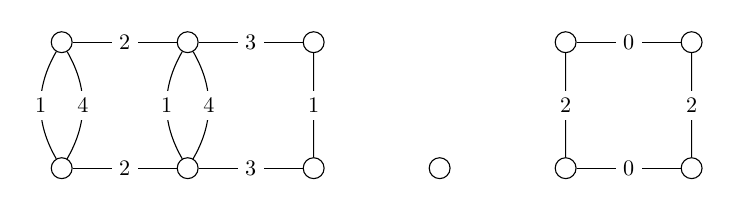
\begin{tikzpicture}[scale=.8]

      \begin{scope}[every node/.style={circle,draw, transform shape}]
        \node (1)  at (0,2)  {};
        \node (2)  at (0,0)  {};
        \node (3)  at (2,2)  {};
        \node (4)  at (2,0)  {};
        \node (5)  at (8,0)  {};
        \node (6)  at (6,0)  {};
        \node (7)  at (8,2)  {};
        \node (8)  at (10,0)  {};
        \node (9)  at (10,2)  {};
        \node (10) at (4,2)  {};
        \node (11) at (4,0) {};
      \end{scope}

      \begin{scope}[every node/.style={fill=white, transform shape}]

        \begin{scope}[every edge/.style={draw}]
          \path (5)  edge node {$0$} (8);
          \path (7)  edge node {$0$} (9);
          \path (1)  edge[bend right=30] node {$1$} (2);
          \path (3)  edge[bend right=30] node {$1$} (4);
          \path (10) edge node {$1$} (11);
          \path (1)  edge node {$2$} (3);
          \path (2)  edge node {$2$} (4);
          \path (5)  edge node {$2$} (7);
          \path (8)  edge node {$2$} (9);
          \path (3)  edge node {$3$} (10);
          \path (4)  edge node {$3$} (11);
          \path (1)  edge[bend left=30] node {$4$} (2);
          \path (3)  edge[bend left=30] node {$4$} (4);
        \end{scope}
      \end{scope}

    \end{tikzpicture}
    \caption{}
  \end{center}
\end{figure}

\paragraph{}This square will consume the last two $\rho_2$ edges. But the component $\{a,b,c,d,e,f\}$ cannot be extend by another alternating square due to the lack of points. Thus it must be connected by a $\rho_2$ edge by Proposition~\ref{square-connection}. But that is impossible and thus the graph can also never be connected.

\paragraph{}
If the two double edges are placed on two different squares, the possibilities for the squares are limited because each square can only contain one $\rho_4$ edge. The single possibility for the square is $[\rho_1, \rho_3]$ by Proposition~\ref{adjacent-squares}. The graph is the following.

\begin{figure}[H]
  \begin{center}
    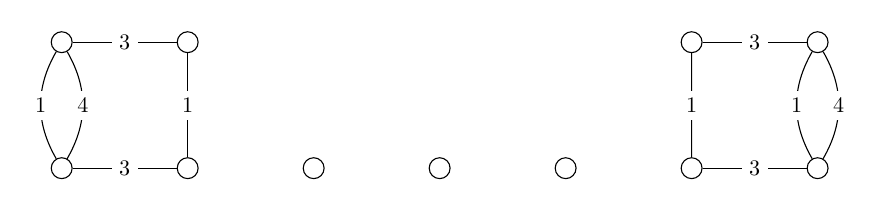
\begin{tikzpicture}[scale=.8]

      \begin{scope}[every node/.style={circle,draw, transform shape}]
        \node (1)  at (0,2)  {};
        \node (2)  at (0,0)  {};
        \node (3)  at (2,2)  {};
        \node (4)  at (2,0)  {};
        \node (5)  at (8,0)  {};
        \node (6)  at (6,0)  {};
        \node (7)  at (12,0)  {};
        \node (8)  at (10,0)  {};
        \node (9)  at (10,2)  {};
        \node (10) at (12,2)  {};
        \node (11) at (4,0) {};
      \end{scope}

      \begin{scope}[every node/.style={fill=white, transform shape}]

        \begin{scope}[every edge/.style={draw}]
          \path (1)  edge[bend right=30] node {$1$} (2);
          \path (3)  edge node {$1$} (4);
          \path (8)  edge node {$1$} (9);
          \path (7)  edge[bend left=30] node {$1$} (10);
          \path (1)  edge node {$3$} (3);
          \path (2)  edge node {$3$} (4);
          \path (8)  edge node {$3$} (7);
          \path (9)  edge node {$3$} (10);
          \path (1)  edge[bend left=30] node {$4$} (2);
          \path (7)  edge[bend right=30] node {$4$} (10);
        \end{scope}
      \end{scope}

    \end{tikzpicture}
    \caption{}
  \end{center}
\end{figure}

\paragraph{}
There are only 4 edges available to connect 5 components. Thus every edge must link two different components. Each square must be linked by a $\rho_2$ edge by Proposition~\ref{square-connection}.

\begin{figure}[H]
  \begin{center}
    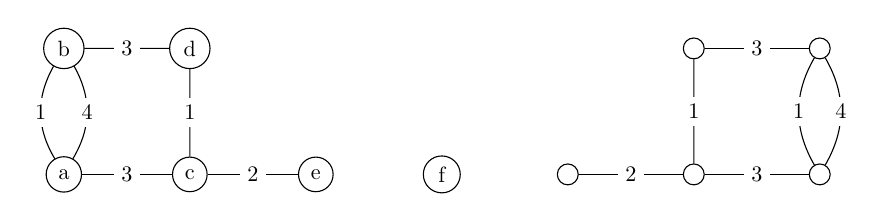
\begin{tikzpicture}[scale=.8]

      \begin{scope}[every node/.style={circle,draw, transform shape}]
        \node (1)  at (0,2)  {b};
        \node (2)  at (0,0)  {a};
        \node (3)  at (2,2)  {d};
        \node (4)  at (2,0)  {c};
        \node (5)  at (8,0)  {};
        \node (6)  at (6,0)  {f};
        \node (7)  at (12,0)  {};
        \node (8)  at (10,0)  {};
        \node (9)  at (10,2)  {};
        \node (10) at (12,2)  {};
        \node (11) at (4,0) {e};
      \end{scope}

      \begin{scope}[every node/.style={fill=white, transform shape}]

        \begin{scope}[every edge/.style={draw}]
          \path (1)  edge[bend right=30] node {$1$} (2);
          \path (3)  edge node {$1$} (4);
          \path (8)  edge node {$1$} (9);
          \path (7)  edge[bend left=30] node {$1$} (10);
          \path (4)  edge node {$2$} (11);
          \path (5)  edge node {$2$} (8);
          \path (1)  edge node {$3$} (3);
          \path (2)  edge node {$3$} (4);
          \path (8)  edge node {$3$} (7);
          \path (9)  edge node {$3$} (10);
          \path (1)  edge[bend left=30] node {$4$} (2);
          \path (7)  edge[bend right=30] node {$4$} (10);
        \end{scope}
      \end{scope}

    \end{tikzpicture}
    \caption{}
  \end{center}
\end{figure}

\paragraph{}
But it is not possible to place the $\rho_0$ edges because they share the vertex $f$ and that is forbidden by Property~\ref{fixed-only-1}.

\end{proof}
